In diesem Kapitel wird die Durchf\"uhrung des Versuches beschrieben.


% **************************************************************************** %
\subsection{Versuchsanordnung}
\label{sec:durchf:subsec:anordn}
% **************************************************************************** %

%\begin{figure}[th!]
%    \centering
%    \includegraphics[width=.5\textwidth]{images/versuchsanordnung.jpeg}
%    \caption{Die Versuchsanordnung}
%\end{figure}
%\begin{figure}[th!]
%    \centering
%    \includegraphics[width=.5\textwidth]{images/blockschaltbild.jpeg}
%    \caption{Die Versuchsanordnung}
%\end{figure}

% Picture and Tools

% **************************************************************************** %
\subsection{Versuchsablauf}
\label{sec:durchf:subsec:ablauf}
% **************************************************************************** %


% ---------------------------------------------------------------------------- %
\subsubsection{Hohlzylinder}
% ---------------------------------------------------------------------------- %

% TODO: Anmerkung shunt-spannung

        \begin{center}
            \captionof{table}{Messwerte Kupferrohr}
            \label{tab:meas:copper}
            \sisetup{math-rm=\mathtt}
            \begin{tabular}{%
                S[table-number-alignment=right]
                S[table-number-alignment=right]
                S[table-number-alignment=right]
                S[table-number-alignment=right]
                }
                \toprule
                {Frequenz ($\si{\hertz}$)}            &
                {Phase ($\si{\degree}$)} &
                {Amplitude ($\si{\milli\volt}$)}      &
                {$V_{R_{Shunt}}$ ($\si{\milli\volt}$)} \\
                \midrule
                   1 &   2   & 70.0 & 195.3 \\
                  10 &  19.2 & 66.0 & 200.0 \\
                  20 &  35.5 & 57.8 & 200.0 \\
                  40 &  56.7 & 41.8 & 200.3 \\
                  80 &  76.7 & 24.4 & 200.0 \\
                 120 &  87   & 16.9 & 200.1 \\
                 160 &  94   & 12.7 & 200.1 \\
                 200 & 100   & 10.0 & 200.0 \\
                 400 & 121   &  4.8 & 200.0 \\
                 600 & 140   &  2.9 & 199.7 \\
                 800 & 155   &  1.9 & 200.5 \\
                1000 & 170   &  1.4 & 200.2 \\
                1200 & 180   &  1.0 & 200.0 \\
                1500 & 200   &  0.7 & 199.9 \\
                \bottomrule
            \end{tabular}
        \end{center}
\begin{figure}[th!]
    \centering
    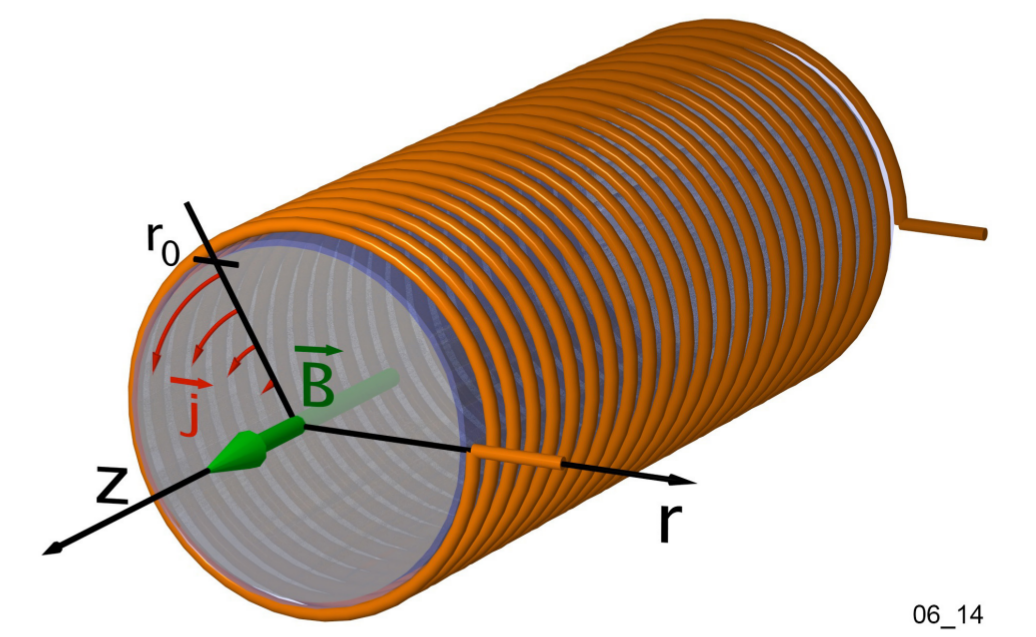
\includegraphics[width=.5\textwidth]{images/spule-vollzylinder.png}
    \caption{Spule mit Vollzylinder \emph{Quelle:} Skript zum Versuch}
\end{figure}


% ---------------------------------------------------------------------------- %
\subsubsection{Vollzylinder}
% ---------------------------------------------------------------------------- %

\begin{figure}[th!]
    \centering
    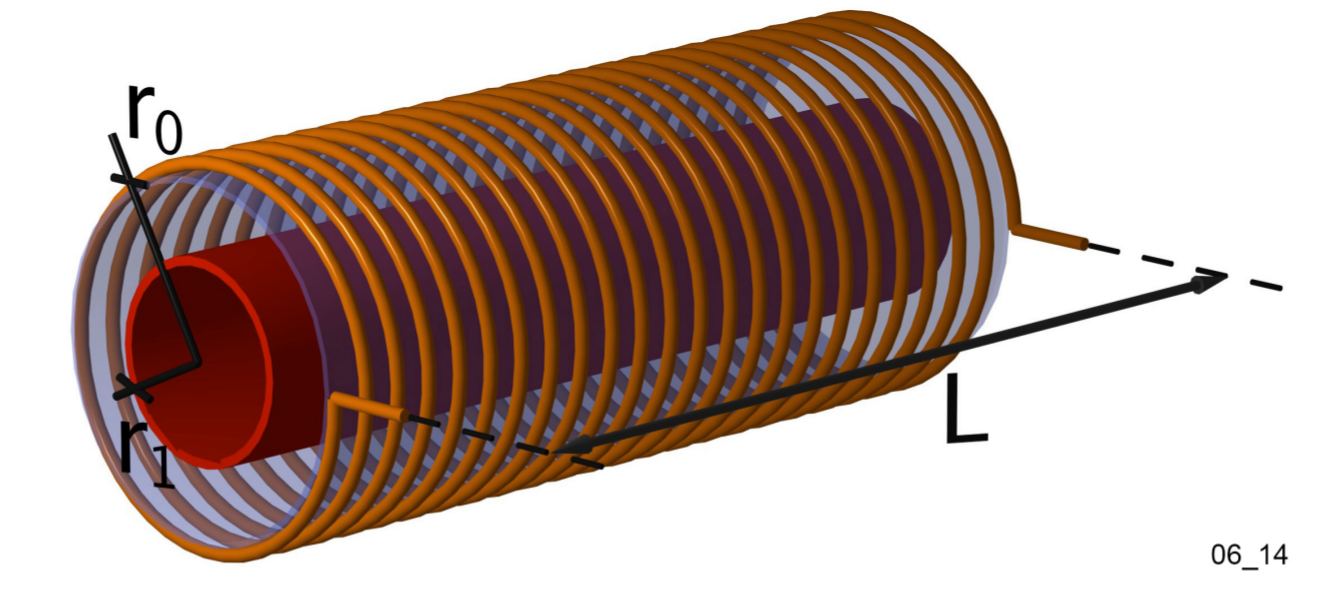
\includegraphics[width=.5\textwidth]{images/spule-hohlzylinder.png}
    \caption{Spule mit Hohlzylinder \emph{Quelle:} Skript zum Versuch}
\end{figure}
